\section{Background Information \& Research}

\subsection{What is Fuzzy Logic?}
Fuzzy logic is a ``natural'' way of expressing uncertain or qualitative information \cite{albertos1998fuzzy}. It is a form of logic that deals with approximate reasoning, as opposed to fixed, exact values, like those found in classical logic (where we may only have properties being true, or false). Instead of these strict truth values, fuzzy logic systems have a range of truth, between 0 and 1. This makes fuzzy logic much better for handling and sorting data, and is an excellent choice for many control system applications, due to the way it mimics human control logic. Lotfi Zadeh, who formalised fuzzy logic in 1965, states that the key advantages of fuzzy logic are that it allows us to make rational decisions in environments of imprecision, uncertainty, and partiality of truth, and to perform a wide variety of physical and mental tasks, without any measurements or computations \cite{zadeh1999computing}.\\[2mm]
\noindent 
In a classical set, the membership, $\mu_A(x)$ of $x$, of a set, $A$, in universe, $X$, is defined:

\begin{center}
\vspace{-3mm}
$ 
\mu_A(x) = \left\lbrace
\begin{array}{ll}
1, & $iff x $\in$ A$      \\
0, & $iff x $\notin$ A$   \\
\end{array} \color{white}\right\rbrace $ 
\end{center}
\vspace{-2mm}
\noindent 
That is, the element is either in the set, or not. In a fuzzy set, however, we have grades of membership, which are real numbers in the interval, $\mu_A(x) \in [0,1]$. Every member of a set has a membership grade to that set, depicting how true the property represented by that set is, for the given member \cite{zadeh1965fuzzy}. The traditional syntax for representing members of a fuzzy set is given below (although a full working knowledge of fuzzy logic theory is not necessary for this project).
\vspace{-2mm}
\begin{center}
$A = \mu_A(x_1)/x_1 + ... + \mu_A(x_n)/x_n$
\end{center}
\vspace{-2mm}
The easiest way to observe the merits of fuzzy logic are to look at terms that we humans use in our everyday life, and attempt to map these are crisp functions. For instances, terms like ``hot'', ``cold'', ``tall'', ``short'', are all terms that we understand very well, and use often. However, if we were asked to give \textit{exact} values for tallness, or shortness, we would not be able to. At what cut-off point would a person change from being considered short, to being considered tall? Fuzzy logic helps to alleviate these impossible choices, by having varying differing degrees of membership, to certain properties. The example in figure \ref{fig:fuzExample} shows this using three linguistic variables to describe the height of a person. Instead of at one point being either tall, short, or medium height, we, at all times, belong to all properties, to a differing degree. 

\begin{figure}[ht!]
\begin{center}
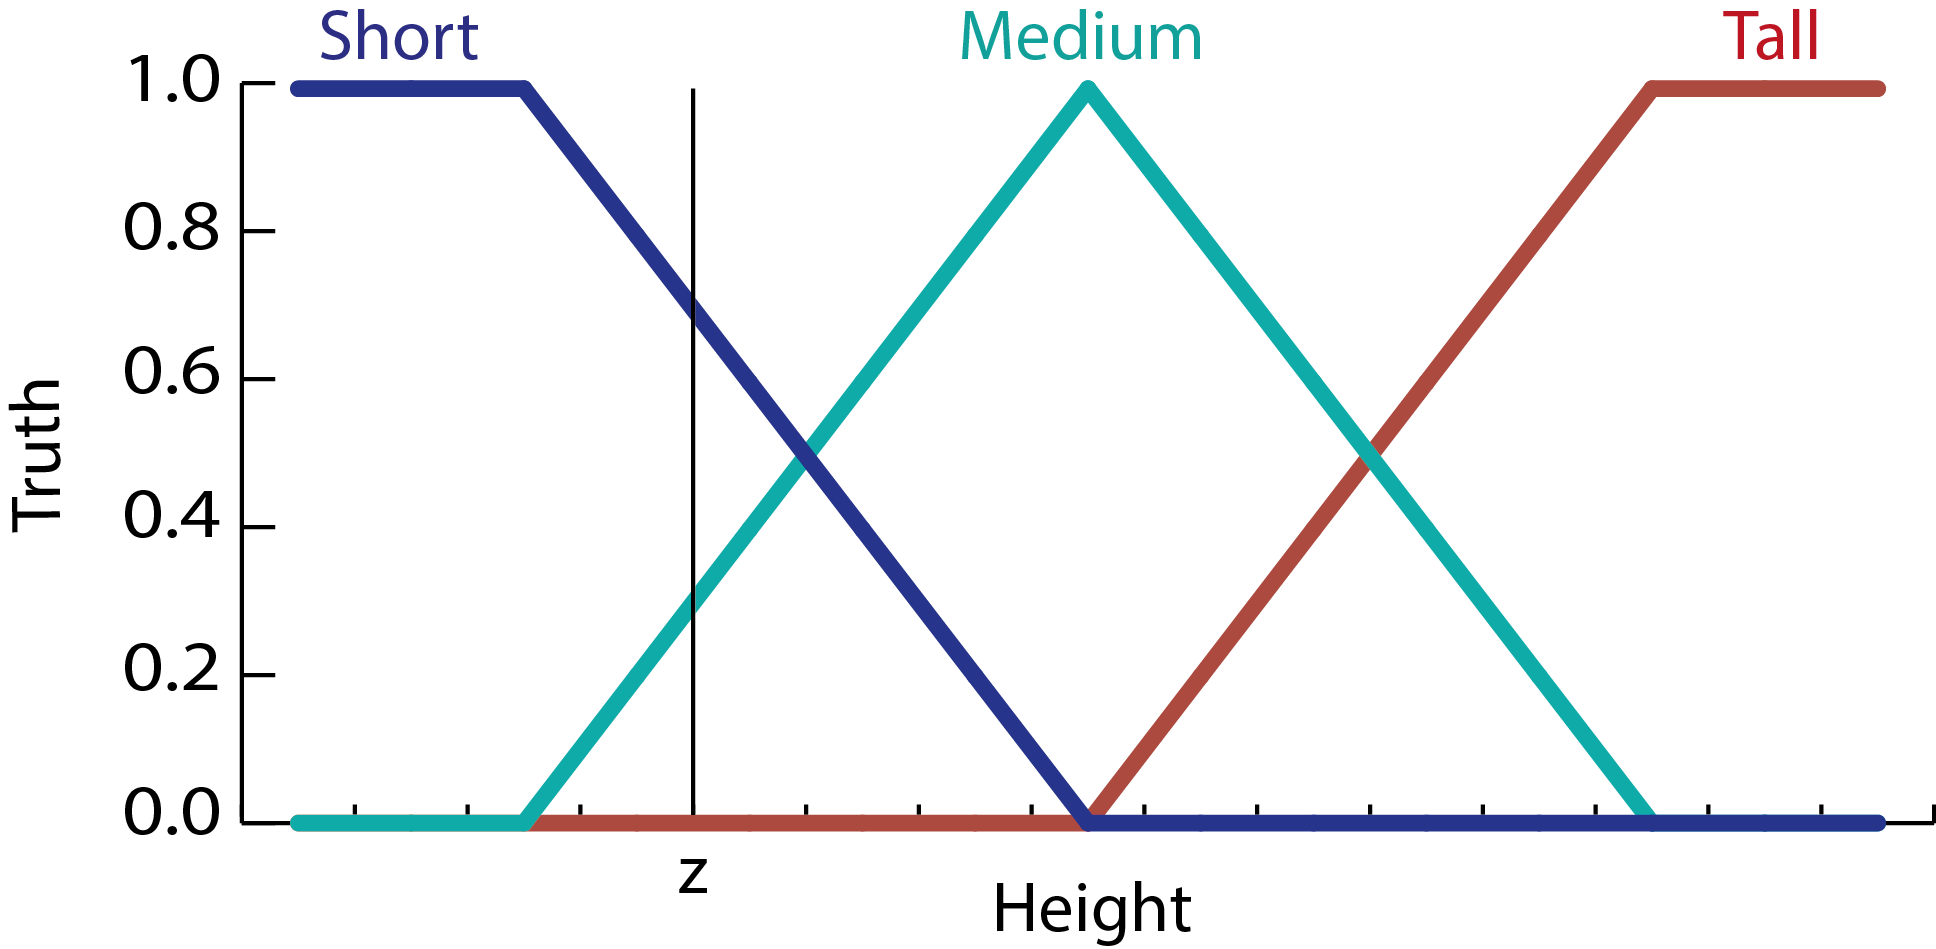
\includegraphics[width=0.6\textwidth]{images/fuzExample.png}
\end{center}
\vspace{-5mm}
\caption{A fuzzy set depicting ``height''}
\label{fig:fuzExample}
\end{figure}
\noindent
For instance, at the point labelled $z$, in the sets in figure \ref{fig:fuzExample}, we belong in the ``Short'' set, to degree 0.7, we belong in the ``Medium'' set, to degree 0.3, and we belong in the ``Tall'' set, to degree 0.0. This is, naturally, much more precise than simply saying we are ``Short'', ``Medium'', or ``Tall''.

\subsection{Existing Systems}
\label{sec:existing-systems}

Fuzzy logic has been around for almost 50 years now, and, with the rising age of the computer, it would be alarming if no software systems for its usage were in circulation. Luckily, this is not the case, and there are many examples of software systems focusing on the use of fuzzy logic, of which many different approaches have been attempted, to varying degrees of success. In this section, a number of these software systems will be evaluated, to discern their positive and negative qualities, to help improve the design of the project presented in this report. 

\paragraph{MATLAB Fuzzy Toolbox}\ \\
The first system to be explored is MATLAB's fuzzy toolbox, an add-on for the MATLAB software suite, to work with fuzzy sets and systems. This toolbox provides everything required to create type-1 fuzzy sets and systems, with relative ease. The main advantage it has over most other systems is that it has a graphical user interface, which makes a tasks like working with fuzzy sets (that require a lot of visualisation and updating in real time) much simpler. There is also an extensive library of documentation and tutorials available for both MATLAB, and this specific toolbox, that help novices to get acquainted with the system. These things both help to make the system very easy to use, and novice friendly.\ \\
\ \\
Unfortunately, these positives do not outweigh the major disadvantage of MATLAB, and the fuzzy toolbox; which is that are pieces of proprietary software. This means that a novice to the field of fuzzy logic would have to invest a considerable sum of money, before they could even begin using the software. Whilst the system does have extensive documentation, and the user would be able to understand and use the system with relative ease, a piece of software does not require a large price tag to achieve this level of functionality and support. Another disadvantage of the MATLAB fuzzy toolbox is that is it not a dedicated piece of software, and is instead a limited subsection of the greater software of MATLAB. This means that the potential for extensibility is much less likely, as updates to the encompassing software would be deemed more important. It could even be argued that the installation of the MATLAB software, and then the installation of further software could be confusing to some novice users, which further alienates them.

\paragraph{FuzzyToolkitUoN}\ \\
FuzzyToolkitUoN is an R-Package, produced by the Intelligent Modelling and Analysis group, at the University of Nottingham, that I personally worked on as part of my Second Year Group Project, at the aforementioned University. It provides functionality for the R Programming language to allow for work with fuzzy sets and fuzzy systems, including their evaluation. A major milestone for the project was it's official acceptance onto CRAN (The Comprehensive R Archive Network, an online library for R packages), in 2013. Being written in R, the package has access to the very powerful R processing tools, and graphics drawing capabilities, which help the user to visualise the system they are creating. Due to being hosted on CRAN, there is extensive documentation for every function in the package, including example usages, and explanations of all their parameters. This makes the usage of the package much simpler, because the user can easily access the documentation for any function they require, and there is a fully worked example for them to follow. Another advantage of the CRAN hosting is that any user with an R interpreter installed can access the package with only a few simple commands, helping the system to be much more accessible.\ \\
\ \\
Unfortunately, there are downsides to working with the R language, the most prominent of which is the command line interface. Whilst the users have the features and functionality to plot the sets they are drawing, it can still be a cumbersome task, and does not promote ease of use. In a graphical user interface, the updating of graphs would be automatic, and the user could see their chances in real time, instead of having to change the graph, and then check what it looked like. Another issue with the package is that the descriptions of the functions, and the system itself, are specified so that a novice to fuzzy logic is not given the support they require; the system assumes that the user's knowledge of fuzzy logic is already somewhat sufficient.

\paragraph{XFuzzy (3.0)}\ \\
Developed by the Institute of Microelectronics in Seville, Spain\footnote{\url{http://www.imse-cnm.csic.es/}}, XFuzzy (3.0), is a set of several tools, that cover the different stages of the creation of a fuzzy system. It allows for the construction of complex systems, whilst also offering flexibility, of allows the user to extend the set of available functions and tools. Each of the tools can be executed as an independent program, or, using the XFuzzy environment, can be integrated together as a graphical user interface, to ease the design process. As mentioned in the evaluation of the MATLAB fuzzy toolbox, a graphical user interface is a huge aid to the user in constructing a fuzzy system, as it allows them to see what changes they are making, and what effect these changes have. The software also runs on Java, which means it can be used on any operating system, as long as the Java Runtime Environment is installed, making it very easy to access. \ \\
\ \\
There are, however, some issues with this software. These being that it is relatively unknown, is not updated frequently (the last update for version 3.0 was in 2012), and without using the graphical user interface, you are stuck using a command line interface, and must learn the system's bespoke language, in order to complete any tasks. The final disadvantage (which is also listed as an advantage, from a different view point), is the necessity for Java to be installed. This is an additional piece of software that this product is dependant on, and could further confuse the novice user with extra installations necessary. 


\paragraph{fuzzyTECH}\ \\
The final system that was observed was fuzzyTECH, another proprietary software, produced by INFORM\footnote{\url{http://www.inform-software.com/}}. It comes with a graphical user interface, making the interaction with the system much simpler than other software available. It also boasts that the application programmer does not require an understanding of fuzzy logic \textit{or} programming to be able to use the system adequately - a feature that the software detailed in this report also hopes to boast. This claim is due to the extensive support functions provided with the software, which can be used to developer software that solves the problem at hand. Another advantage of fuzzyTECH is that is produces source code that can be used on various hardware platforms (for instance, PCs and micro-controllers).
\ \\
\ \\
The disadvantages of fuzzyTECH, just as with the MATLAB fuzzy toolbox, is that it is a pay-to-use piece of software. This greatly alienates the novice user, as they may not be willing to spend a large sum of money on a software they have never used, for a purpose they have never experienced before. There are also many different versions of fuzzyTECH, which would further confuse the novice user, as they may not necessary be aware of their specific needs, and thus be unsure as to which specific version would suit them best. In addition to this, fuzzyTECH has not been updated since early 2010, meaning the support that the novice user requires, may not be there - despite the systems extensive support functions. 







{\color{red}
Talk about fuzzy toolkituon, matlab, xfuzzy (brief), fuzzytech(brief), mention their positions and negatives in terms of the key flaws, and novice users.\ \\
\ \\
Then talk about my project and how this will counter the specific issues raised.
}


\subsection{Platforms and Tools}
{\color{red}\begin{enumerate}
\item Languages used (R, Javascript)
\item Web technologies (tools, languages)
\item Shiny r to html
\item Bootstrap
\item jquery
\item Good user interfaces
\end{enumerate}}

